\documentclass[10pt,a4paper]{article}
\usepackage[utf8]{inputenc} 
\usepackage[spanish]{babel}
\usepackage{a4wide}
\usepackage{float}
\usepackage{caratula}

\begin{document}

\titulo{Trabajo Práctico}
\subtitulo{SLS: Un simple lenguaje de scripting}

\fecha{\today}

\materia{Teoría de Lenguajes}
\grupo{Los Libres de Contexto}

\integrante{Castro, Alan}{356/10}{alancastro90@gmail.com}
\integrante{Bonomi, Cyntia}{134/03}{cyntiab83@gmail.com}
\integrante{Izcovich, Sabrina}{550/11}{sizcovich@gmail.com}

\maketitle

\tableofcontents

\newpage
\section{Introducción}

\section{Gramática}

En lo que sigue, presentamos la gramática utilizada para la realización del parser:\\

PROGRAM $\rightarrow$ LIST\_SENTENCIES \\

LIST\_SENTENCIES $\rightarrow$ SENTENCE $|$ SENTENCE LIST\_SENTENCIES\\

SENTENCE $\rightarrow$ E; $|$ WHILE $|$ IF\_ELSE $|$ CONDITIONAL $|$ FOR $|$ DO\_WHILE $|$ COMMENT \\

WHILE $\rightarrow$ while (CONDITION) SENTENCE $|$ while (CONDITION) {LIST\_SENTENCIES} \\

IF\_ELSE $\rightarrow$ IF else SENTENCE $|$ IF else {LIST\_SENTENCIES} \\

IF $\rightarrow$ if (CONDITION) SENTENCE $|$ if (CONDITION) {LIST\_SENTENCIES} \\

CONDITIONAL $\rightarrow$ (CONDITION) ? SENTENCE : SENTENCE \\

FOR $\rightarrow$ for(ASIGNACION ;CONDITION; AVANZAR) SENTENCE $|$ (ASIGNACION ;CONDITION; AVANZAR) {LIST\_SENTENCIES} \\

ASIGNACION $\rightarrow$ $\lambda$ $|$ var = EXPRESSION $|$ var[NUM] = EXPRESSION $|$ var[NUM] = EXPRESSION\\

AVANZAR $\rightarrow$ var++ $|$ var$--$ $|$ var -= NUM $|$ var += NUM $|$ $\lambda$ \\

DO\_WHILE $\rightarrow$ do LIST\_SENTENCIES while (CONDITION) \\

CONDITION $\rightarrow$ LOGICAL\_CONDITION $|$ CONDITION\_AND $|$ CONDITION\_OR \\

CONDITION\_AND $\rightarrow$ LOGICAL\_CONDITION AND LOGICAL\_CONDITION \\

CONDITION\_OR $\rightarrow$ LOGICAL\_CONDITION OR LOGICAL\_CONDITION \\

LOGICAL\_CONDITION $\rightarrow$ E $>$ E $|$ E $<$ E $|$ E == E $|$ E != E \\

E $\rightarrow$ ASIGNACION $|$ EXPRESSION \\

VALUE $\rightarrow$ string $|$ bool $|$ var $|$ NUM $|$FUNCION $|$ var[NUM] $|$ [LIST\_VALUES] $|$ LIST\_REGISTERS\\

LIST\_REGISTERS $\rightarrow$ REGISTER $|$ REGISTER , LIST\_REGISTERS\\

REGISTER $\rightarrow$ cadena:VALUE \\

LIST\_VALUES $\rightarrow$ VALUE $|$ VALUE , LIST\_VALUES \\

EXPRESSION $\rightarrow$  ARITHMETIC\_EXPRESSION $|$ VALUE \\

FUNCTION $\rightarrow$ FUNCTION\_WITH\_RETURN $|$ FUNCTION\_NO\_RETURN \\

FUNCTION\_WITH\_RETURN $\rightarrow$ multiplicacionEscalar(PARAM\_ME) $|$  capitalizar(string) $|$  colineales(var, var) $|$ length(PARAM\_LENGTH) \\

FUNCTION\_NO\_RETURN $\rightarrow$ print(EXPRESSION) \\

PARAM\_ME $\rightarrow$ var, NUM, bool $|$ var, NUM \\

PARAM\_LENGTH $\rightarrow$ var $|$ string \\

LIST\_PARAMETROS $\rightarrow$ EXPRESSION $|$ LIST\_PARAMETROS , EXPRESSION \\

ARITHMETIC\_EXPRESSION $\rightarrow$  + TERM $|$ ARITHMETIC\_EXPRESSION - TERM $|$ TERM \\

TERM $\rightarrow$ TERM $*$ FACTOR $|$ TERM $/$ FACTOR $|$ TERM \% FACTOR $|$ FACTOR \\

FACTOR $\rightarrow$ NUM $|$ var[NUM] \\

NUM $\rightarrow$ decimal $|$ natural


\section{Gramática de Atributos}

\subsection{Inicio del programa}
\textbf{PROGRAM} $\rightarrow$ \textbf{LIST\_SENTENCIES} \\
\textit{\{LIST\_SENTENCIES.level = 0, PROGRAM.value = LIST\_SENTENCIES.value, print(PROGRAM.value)\}}\\

\textbf{LIST\_SENTENCIES} $\rightarrow$ \textbf{G A}\\
\textit{\{G.level = LIST\_SENTENCIES.level, A.level = LIST\_SENTENCIES.level, LIST\_SENTENCIES.value = IF(G.value==' ' , ' ', G.value + '$\setminus$n') + A.value, LIST\_SENTENCIES.element = G.element, A.element = G.element\}} \\

\textbf{G} $\rightarrow$ \textbf{comment} \\
\textit{\{G.value = comment.value + '$\setminus$n'\}} \\
G.element = 'comment'

\textbf{G} $\rightarrow$ \textbf{SENTENCE} \\
\textit{\{G.value = indent(G.level) + SENTENCE.value, SENTENCE.level = G.level\}} \\

\textbf{G} $\rightarrow$ newline \\
\textit{\{G.value = ' '\}} \\

\textbf{A} $\rightarrow$ \textbf{LIST\_SENTENCIES}\\
\textit{\{LIST\_SENTENCIES.level = A.level, A.value = IF(((LIST\_SENTENCIES.element == 'sentence' $||$ LIST\_SENTENCIES.element == 'newline') \&\& A.element == 'sentence') $||$ A.element == 'comment', '$\setminus$n') + LIST\_SENTENCIES.value\}} \\

\textbf{A} $\rightarrow$ $\lambda$ \\
\textit{\{A.value = '$\setminus$n'\}} \\

\subsection{Sentencias}
\textbf{SENTENCE} $\rightarrow$ \textbf{E};\\ 
\textit{\{E.level = SENTENCE.level, SENTENCE.value = E.value + ';'\}} \\

\textbf{SENTENCE} $\rightarrow$ \textbf{WHILE} \\ 
\textit{\{WHILE.level = SENTENCE.level, SENTENCE.value = WHILE.value\}} \\

\textbf{SENTENCE} $\rightarrow$ \textbf{IF\_ELSE}  \\ 
\textit{\{IF\_ELSE.level = SENTENCE.level, SENTENCE.value = IF\_ELSE.value\}} \\

\textbf{SENTENCE} $\rightarrow$ \textbf{FOR} \\ 
\textit{\{FOR.level = SENTENCE.level, SENTENCE.value = FOR.value\}} \\

\textbf{SENTENCE} $\rightarrow$ \textbf{DO\_WHILE} \\ 
\textit{\{DO\_WHILE.level = SENTENCE.level, SENTENCE.value = DO\_WHILE.value\}}  \\

\textbf{SENTENCE} $\rightarrow$ \textbf{FUNCTION}; \textbf{POSSIBLECOMMENT} \\
\textit{\{FUNCTION.level = SENTENCE.level, SENTENCE.value = FUNCTION.value + ';' + POSSIBLECOMMENT.value\}} \\

\subsection{Terminados en ;}

\textbf{E} $\rightarrow$ \textbf{ASSIGNATION}\\
\textit{\{E.value = ASSIGNATION.value\}}\\

\textbf{E} $\rightarrow$ \textbf{EXPRESSION} \\
\textit{\{E.value = EXPRESSION.value\}} \\

\textbf{E} $\rightarrow$ \textbf{CONDITIONAL} \\
\textit{\{E.value = CONDITIONAL.value\}} \\

\subsection{Comentarios}

\textbf{POSSIBLECOMMENT} $\rightarrow$ comment \\
\textit{\{POSSIBLECOMMENT.value = comment.value\}} \\

\textbf{POSSIBLECOMMENT} $\rightarrow$ $\lambda$ \\
\textit{\{POSSIBLECOMMENT.value = ' '\}} \\

\textbf{$COMMENT\_LIST_{1}$} $\rightarrow$ comment \textbf{$COMMENT\_LIST_{2}$} \\
\textit{\{$COMMENT\_LIST_{1}$.value = comment.value + '$\setminus$n' + $COMMENT\_LIST_{2}$\}} \\

\textbf{$COMMENT\_LIST_{1}$} $\rightarrow$ newline \textbf{$COMMENT\_LIST_{2}$} \\
\textit{\{$COMMENT\_LIST_{1}$.value = '$\setminus$n' + $COMMENT\_LIST_{2}$\}} \\

\textbf{COMMENT\_LIST} $\rightarrow$ $\lambda$ \\
\textit{\{COMMENT\_LIST.value = ' '\}} \\

\subsection{Estructuras de control}
\textbf{WHILE} $\rightarrow$ while (\textbf{CONDITION}) \textbf{POSSIBLECOMMENT KEYS} \\
\textit{\{KEYS.level = WHILE.level + 1, WHILE.value = indent(WHILE.level) + 'while (' + CONDITION.value + ') ' + POSSIBLECOMMENT.value + '$\setminus$n' + KEYS.value\}} \\

\textbf{IF\_ELSE} $\rightarrow$ \textbf{IF} else \textbf{POSSIBLECOMMENT KEYS} \\
\textit{\{KEYS.level = IF\_ELSE.level + 1, IF\_ELSE.value = indent(IF\_ELSE.level) + IF.value + 'else' + POSSIBLECOMMENT.value + '$\setminus$n' + KEYS.value\}} \\

\textbf{IF} $\rightarrow$ if (\textbf{CONDITION}) \textbf{POSSIBLECOMMENT KEYS} \\
\textit{\{KEYS.level = IF.level + 1, IF.value = 'if (' + CONDITION.value + ') ' + POSSIBLECOMMENT.value + '$\setminus$n' + KEYS.value\}} \\

\textbf{CONDITIONAL} $\rightarrow$ (\textbf{CONDITION}) ? \textbf{$EXPRESSION_{1}$} : \textbf{$EXPRESSION_{2}$}  \\
\textit{\{CONDITIONAL.value = '(' + CONDITION.value + ')?' + $EXPRESSION_{1}$.value + ':' + $EXPRESSION_{2}$.value\}}\\
	
\textbf{FOR} $\rightarrow$ for(\textbf{ASSIGNATIONORLAMBDA}; \textbf{CONDITION}; \textbf{ADVANCE}) \textbf{POSSIBLECOMMENT KEYS}  \\
\textit{\{KEYS.level = FOR.level + 1, FOR.value = indent(FOR.level) + 'for (' + ASSIGNATIONORLAMBDA.value + ';' + CONDITION.value + ';' + ADVANCE.value ') ' + POSSIBLECOMMENT.value + '$\setminus$n' + KEYS.value\}}\\

\textbf{DO\_WHILE} $\rightarrow$ do \{\textbf{$POSSIBLECOMMENT_{1}$ LIST\_SENTENCIES}\} while (\textbf{CONDITION}); \textbf{$POSSIBLECOMMENT_{2}$} \\
\textit{\{LIST\_SENTENCIES.level = DO\_WHILE.level + 1, DO\_WHILE.value = indent(DO\_WHILE.level) + 'do{' + $POSSIBLECOMMENT_{1}$.value + '$\setminus$n' + LIST\_SENTENCIES.value + '} while(' + CONDITION.value + '); ' + $POSSIBLECOMMENT_{2}$.value + '$\setminus$n'\}}\\

\textbf{KEYS} $\rightarrow$ \textbf{COMMENT\_LIST SENTENCE} \\ 
\textit{\{COMMENT\_LIST.level = KEYS.level, SENTENCE.level = KEYS.level, KEYS.value = COMMENT\_LIST.value + indent(KEYS.level) + SENTENCE.value\}} \\

\textbf{KEYS} $\rightarrow$ \{ \textbf{POSSIBLECOMMENT} \textbf{LIST\_SENTENCIES} \} \\
\textit{\{LIST\_SENTENCIES.level = KEYS.level, KEYS.value = '\{' + POSSIBLECOMMENT.value + '$\setminus$n' + LIST\_SENTENCIES.value + '\}' + '$\setminus$n'\}} \\

\subsection{Asignaciones}


\textbf{ASSIGNATIONORLAMBDA} $\rightarrow$ \textbf{ASSIGNATION} \\
\textit{\{ASSIGNATIONORLAMBDA.value = ASSIGNATION.value\}} \\

\textbf{ASSIGNATIONORLAMBDA} $\rightarrow$ $\lambda$ \\
\textit{\{ASSIGNATIONORLAMBDA.value = ' '\}} \\

\textbf{ASSIGNATION} $\rightarrow$ var \textbf{B} \\
\textit{\{ASSIGNATION.value = var.value + B.value, 
IF(B.isArray, COND(table(var.value) != None \&\& table.getType(var.value) == B.type \&\& B.isArray==table.isArray(var.value)), table.insertOrUpdate(var.value, B.type, B.isArray)\}} \\

\textbf{B} $\rightarrow$ [natural] = \textbf{EXPRESSION}  \\
\textit{\{B.value = '[' + natural.value + '] = ' + EXPRESSION.value, B.type = IF(EXPRESSION.type == 'natural', 'decimal', EXPRESSION.type), B.isArray = true\}} \\

\textbf{B} $\rightarrow$ = \textbf{EXPRESSION} \\
\textit{\{B.value = '=' + EXPRESSION.value, B.type = EXPRESSION.type, B.isArray = false\}} \\

\subsection{Avanzar}
\textbf{ADVANCE} $\rightarrow$ var \textbf{C} \\
\textit{\{COND(var.type == NUM), ADVANCE.value = var.value + C.value\}} \\

\textbf{ADVANCE} $\rightarrow$ $\lambda$ \\
\textit{\{ADVANCE.value = ' '\}} \\

\subsection{Incremento y Decremento}
\textbf{C} $\rightarrow$ +\textbf{D} \\ 
\textit{\{ C.value = '+' + D.value   \}} \\

\textbf{C} $\rightarrow$ -\textbf{F} \\
\textit{\{ C.value = '-' + F.value   \}} \\

\textbf{D} $\rightarrow$ +   \\
\textit{\{ D.value = '+'  \}} \\

\textbf{D} $\rightarrow$ = \textbf{NUM} \\
\textit{\{ D.value =  '=' + NUM.value  \}} \\

\textbf{F} $\rightarrow$ - \\
\textit{\{ F.value = '-'  \}} \\

\textbf{F} $\rightarrow$ = \textbf{NUM} \\
\textit{\{ F.value =  '=' + NUM.value\}} \\

\subsection{Condiciones}
\textbf{CONDITION} $\rightarrow$ \textbf{LOGICAL\_CONDITION}   \\
\textit{\{CONDITION.value = LOGICAL\_CONDITION.value\}}\\

\textbf{CONDITION} $\rightarrow$ \textbf{BOOLEAN\_CONDITION} \\
\textit{\{ CONDITION.value = BOOLEAN\_CONDITION.value\}} \\

\textbf{BOOLEAN\_CONDITION} $\rightarrow$ \textbf{LOGICAL\_CONDITION H} \\
\textit{\{BOOLEAN\_CONDITION.value = LOGICAL\_CONDITION + H.value\}} \\

\textbf{H} $\rightarrow$ and \textbf{BOOLEAN\_CONDITION} \\
\textit{\{ H.value = 'and' + BOOLEAN\_CONDITION.value\}} \\

\textbf{H} $\rightarrow$ or \textbf{BOOLEAN\_CONDITION} \\
\textit{\{ H.value = 'or' + BOOLEAN\_CONDITION.value\}} \\

\textbf{H} $\rightarrow$ $lambda$ \\
\textit{\{H.value = ' '\}} \\

\textbf{LOGICAL\_CONDITION} $\rightarrow$ \textbf{E I} \\
\textit{\{ LOGICAL\_CONDITION.value = E.value + I.value\}} \\

\subsection{Comparaciones}
\textbf{I} $\rightarrow$ $>$ \textbf{E} \\
\textit{\{ I.value = '$>$' + E.value  \}} \\

\textbf{I} $\rightarrow$ $<$ \textbf{E}\\
\textit{\{ I.value = '$<$' + E.value  \}} \\

\textbf{I} $\rightarrow$ $==$ \textbf{E}\\
\textit{\{ I.value =  '==' + E.value\}} \\

\textbf{I} $\rightarrow$ $!=$ \textbf{E}\\
\textit{\{ I.value =  '!=' + E.value\}} \\

\subsection{Valores}
\textbf{VALUE} $\rightarrow$ string \\
\textit{\{VALUE.value = string.value, VALUE.type = 'string'\}} \\

\textbf{VALUE} $\rightarrow$ bool   \\
\textit{\{VALUE.value = bool.value, VALUE.type = 'bool'\}} \\

\textbf{VALUE} $\rightarrow$ \textbf{NUM}   \\
\textit{\{VALUE.value =  NUM.value , VALUE.type =  NUM.type\}} \\

\textbf{VALUE} $\rightarrow$ \textbf{FUNCTION\_WITH\_RETURN} \\
\textit{\{VALUE.value =  FUNCTION\_WITH\_RETURN.value, VALUE.type = FUNCTION\_WITH\_RETURN.type\}} \\

\textbf{$VALUE_1$} $\rightarrow$ [\textbf{$VALUE_2$ LIST\_VALUES}]   \\
\textit{\{$VALUE_1$.value =  '[ ' + $VALUE_2$.value + LIST\_VALUES.value + ']', LIST\_VALUES.type = IF($VALUE_2$.type == 'natural','decimal',$VALUE_2$.type), $VALUE_1$.type = $VALUE_2$.type\}} \\

\textbf{VALUE} $\rightarrow$ \{\textbf{LIST\_REGISTERS}\} \\
\textit{\{VALUE.value =  LIST\_REGISTERS.value , VALUE.type = 'register'\}} \\

\textbf{VALUE} $\rightarrow$ var \textbf{J} \\
\textit{\{VALUE.value =  var.value + J.value, VALUE.type = IF(J.isArray, table.getType(var.value), var.type)\}} \\

\textbf{J} $\rightarrow$ [\textbf{NUM}] \\
\textit{\{J.value = '[' + NUM.value + ']', J.isArray = true   \}} \\

\textbf{J} $\rightarrow$ $\lambda$   \\
\textit{\{J.value = ' ', J.isArray = false\}} \\

\subsection{Listas}
\textbf{LIST\_REGISTERS} $\rightarrow$ \textbf{ASSIGNATION L} \\
\textit{\{LIST\_REGISTERS.value = ASSIGNATION.value + L.value\}} \\

\textbf{L} $\rightarrow$, \textbf{LIST\_REGISTERS} \\
\textit{\{L.value = ',' + LIST\_REGISTERS.value\}} \\

\textbf{L} $\rightarrow$ $\lambda$\\
\textit{\{LIST\_REGISTERS.value =  ' ' \}}  \\ 

\textbf{$LIST\_VALUES_1$} $\rightarrow$ \textbf{, VALUE $LIST\_VALUES_2$} \\
\textit{\{$LIST\_VALUES_1$.value =  ',' + VALUE.value + $LIST\_VALUES_2$.value, $LIST\_VALUES_1$.type = $LIST\_VALUES_2$.type, COND($LIST\_VALUES_2$.type == IF(VALUE.type == 'natural','decimal',VALUE.type))\}} \\

\textbf{LIST\_VALUES} $\rightarrow$ $\lambda$ \\
\textit{\{LIST\_VALUES.value = ' '\}} \\

\subsection{Expresiones}
\textbf{EXPRESSION} $\rightarrow$ \textbf{ARITHMETIC\_EXPRESSION} \\   
\textit{\{EXPRESSION.value =  ARITHMETIC\_EXPRESSION.value, EXPRESSION.type = ARITHMETIC\_EXPRESSION.type \}}  \\

\textbf{EXPRESSION} $\rightarrow$ \textbf{EXPRESSION\_STRING} \\
\textit{\{EXPRESSION.value =  EXPRESSION\_STRING.value, EXPRESSION.type = 'string' \}}  \\ 

\textbf{EXPRESSION} $\rightarrow$ \textbf{VALUE} \\
\textit{\{EXPRESSION.value =  VALUE.value, EXPRESSION.type = VALUE.type \}} \\

\textbf{$EXPRESSION\_STRING_1$} $\rightarrow$ \textbf{$EXPRESSION\_STRING_2$} + \textbf{string} \\ \textit{\{$EXPRESSION\_STRING_1$.value =  $EXPRESSION\_STRING_2$.value + '+' + string.value\}} \\

\textbf{$ARITHMETIC\_EXPRESSION_1$} $\rightarrow$ \textbf{$ARITHMETIC\_EXPRESSION_2$} + \textbf{TERM} \\
\textit{\{$ARITHMETIC\_EXPRESSION_1$.value = $ARITHMETIC\_EXPRESSION_2$.value + '+' + TERM.value, $ARITHMETIC\_EXPRESSION_2$.type = TERM.type\}} \\

\textbf{$ARITHMETIC\_EXPRESSION_1$} $\rightarrow$ \textbf{$ARITHMETIC\_EXPRESSION_2$} - \textbf{TERM}  \\
\textit{\{$ARITHMETIC\_EXPRESSION_1$.value = $ARITHMETIC\_EXPRESSION_2$.value + '-' + TERM.value, $ARITHMETIC\_EXPRESSION_1$.type = TERM.type\}} \\

\textbf{ARITHMETIC\_EXPRESSION} $\rightarrow$ \textbf{TERM} \\
\textit{\{ARITHMETIC\_EXPRESSION.value = TERM.value, ARITHMETIC\_EXPRESSION.type = TERM.type\}}  \\

\subsection{Términos}
\textbf{TERM} $\rightarrow$ \textbf{$TERM_{1}$} $*$ \textbf{FACTOR}   \\
\textit{\{TERM.value = $TERM_{1}$.value + '$*$' + FACTOR.value, TERM.type = FACTOR.type\}} \\

\textbf{TERM} $\rightarrow$ \textbf{$TERM_{1}$} $/$ \textbf{FACTOR}   \\
\textit{\{TERM.value = $TERM_{1}$.value + '$/$' + FACTOR.value, TERM.type = FACTOR.type\}} \\

\textbf{TERM} $\rightarrow$ \textbf{$TERM_{1}$} \% \textbf{FACTOR}  \\
\textit{\{TERM.value = $TERM_{1}$.value + '\%' + FACTOR.value, TERM.type = FACTOR.type\}} \\

\textbf{TERM} $\rightarrow$ \textbf{FACTOR} \\
\textit{\{TERM.value = FACTOR.value, TERM.type = FACTOR.type\}} \\

\textbf{FACTOR} $\rightarrow$ \textbf{NUM}   \\
\textit{\{FACTOR.value = NUM.value, FACTOR.type = 'decimal'\}} \\

\textbf{FACTOR} $\rightarrow$ var[\textbf{NUM}]  \\ 
\textit{\{FACTOR.value = var.value + '[' + NUM.value + ']', FACTOR.type = 'decimal', COND(NUM.type == 'natural'), COND(table.getType(var.value) == 'natural' $||$ table.getType(var.value) == 'decimal')\}}  \\ 
\\

\subsection{Funciones}
\textbf{FUNCTION} $\rightarrow$ \textbf{FUNCTION\_WITH\_RETURN} \\
\textit{\{FUNCTION.value =  FUNCTION\_WITH\_RETURN.value, FUNCTION.type = FUNCTION\_WITH\_RETURN.type\}} \\

\textbf{FUNCTION} $\rightarrow$ print(\textbf{EXPRESSION}) \\   
\textit{\{FUNCTION.value =  'print(' + EXPRESSION.value + ')', FUNCTION.type = 'void'\}} \\

\textbf{FUNCTION\_WITH\_RETURN} $\rightarrow$ multiplicacionEscalar(\textbf{PARAM\_ME}) \\ 
\textit{\{FUNCTION\_WITH\_RETURN.value =  'multiplicacionEscalar(' + PARAM\_ME.value + ')', , FUNCTION\_WITH\_RETURN.type = PARAM\_ME.type\}} \\

\textbf{FUNCTION\_WITH\_RETURN} $\rightarrow$ capitalizar(string)   \\
\textit{\{FUNCTION\_WITH\_RETURN.value =  'capitalizar(' + string.value + ')', FUNCTION\_WITH\_RETURN.type = 'string'\}} \\

\textbf{FUNCTION\_WITH\_RETURN} $\rightarrow$ colineales($var_{1}$, $var_{2}$)   \\
\textit{\{COND((table.getType($var_{1}$.value) == natural $||$ table.getType($var_{1}$.value) == 'decimal' \&\& table.isArray($var_{1}$.value) \&\& table.isArray($var_{2}$.value)) \&\&
(table.getType($var_{2}$.value) == 'natural' $||$ table.getType($var_{2}$.value) == 'decimal')), FUNCTION\_WITH\_RETURN.value = 'colineales (' + $var_{1}$.value + ', ' +$var_{2}$.value')', FUNCTION\_WITH\_RETURN.type = 'bool' \}} \\

\textbf{FUNCTION\_WITH\_RETURN} $\rightarrow$ length(\textbf{PARAM\_LENGTH}) \\
\textit{\{FUNCTION\_WITH\_RETURN.value =  'length(' + PARAM\_LENGTH.value + ')',\\ 
FUNCTION\_WITH\_RETURN.type = 'natural'\}} \\

\subsection{Parámetros de funciones}
\textbf{PARAM\_ME} $\rightarrow$ var, \textbf{NUM N} \\
\textit{\{ PARAM\_ME.value = var.value + ',' + NUM.value + N.value, COND(table.getType(var.value) == 'natural' $||$ table.getType(var.value) == 'decimal'), COND(table.isArray(var.value)),\\
PARAM\_ME.type = IF(table.getType(var.value) == 'decimal' \&\& N.isTrue,  'natural' , table.getType(var.value))\}} \\

\textbf{N} $\rightarrow$ ,\textbf{BOOL} \\
\textit{\{ N.value = ', bool', N.isTrue = N.value\}} \\ 

\textbf{N} $\rightarrow$ $lambda$  \\
\textit{\{N.value = ' ', N.isTrue = false\}} \\

\textbf{PARAM\_LENGTH} $\rightarrow$ var \\
\textit{\{PARAM\_LENGTH.value = var.value, COND(table.isArray(var.value) $||$ (table.getType(var.value) == 'string'))\}} \\

\textbf{PARAM\_LENGTH} $\rightarrow$ [VALUE LIST\_VALUES]\\
\textit{\{PARAM\_LENGTH.value = '[' + VALUE.value + LIST\_VALUES.value + ']', LIST\_VALUES.type = IF(VALUE.type == 'natural','decimal',VALUE.type)\}} \\

\textbf{PARAM\_LENGTH} $\rightarrow$ string \\
\textit{\{PARAM\_LENGTH.value = string.value\}} \\

\subsection{Tipos numéricos}
\textbf{NUM} $\rightarrow$ decimal \\
\textit{\{NUM.value = decimal.value, NUM.type = 'decimal')\}}  \\ 

\textbf{NUM} $\rightarrow$ natural \\
\textit{\{NUM.value = natural.value, NUM.type = 'natural')\}}  \\ 

\subsection{Tipos Booleanos}
\textbf{BOOL} $\rightarrow$ true \\
\textit{\{ BOOL.value = 'true' \}} \\ 

\textbf{BOOL} $\rightarrow$ false \\
\textit{\{ BOOL.value = 'false' \}} \\ 


\subsection{Atributos}

\begin{itemize}
\item Terminales natural.value, decimal.value, string.value
\item \textbf{PARAM\_LENGTH.value, NUM.value:} string (\textit{sintetizado}) es el código de salida del parser arreglado.
\item \textbf{Level:} int (\textit{heredado}) almacena el nivel de indentación de la producción actual.
\item \textbf{NUM.type:} string (\textit{sintetizado}) representa el tipo de la expresión en cuestión.
\item \textbf{N.isTrue:} bool (\textit{sintetizado}) almacena la información del booleano dado por parámetro en multiplicacionEscalar.
\end{itemize}

\section{Ejemplo de la Gramática de Atributos}

\begin{figure}[H]
\begin{center}
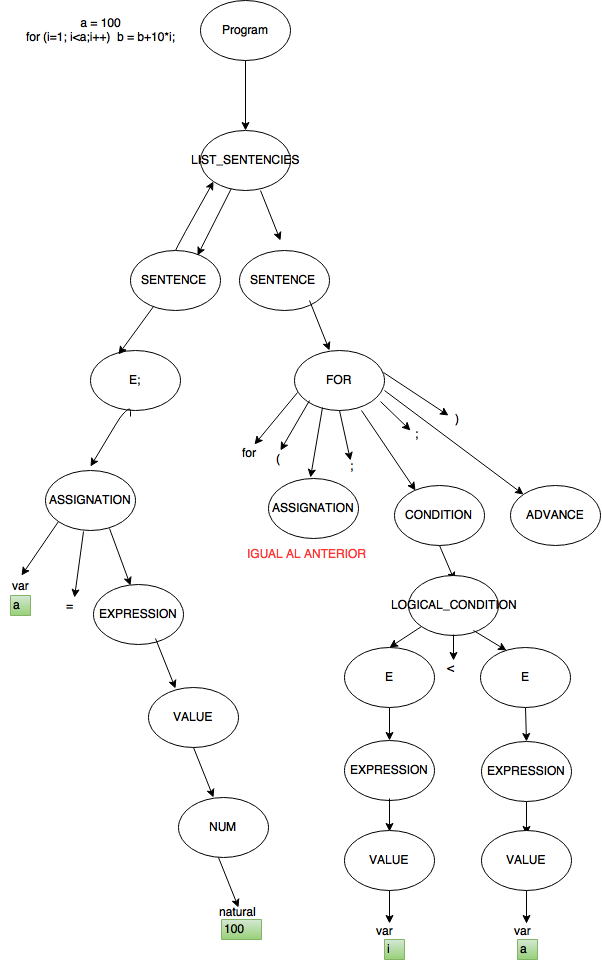
\includegraphics[scale=0.7]{imgs/ejemploGramatica.png}
\end{center}
\end{figure}

En el diagrama anterior, se pueden observar las derivaciones de una parte del programa presentado a modo de ejemplo.

\section{Descripción}

Para la realización de nuestro trabajo práctico, tomamos las siguientes decisiones:
\begin{itemize}
\item En la gramática, nuestro diccionario está en $R^2$ 

\item x.valor + y.valor representa la concatenación

\item Por defecto, los arreglos se inicializan como decimales si son números

\item Asumimos que ASIGNACION $\rightarrow$ VAR = NUM 

\item Asumimos que los Registers toman únicamente literales de tipos básicos.

\item Decidimos que los comentarios se reescriben en la línea de abajo para mayor claridad del código.

\item El único newline que nos interesa es entre \{ ; \{ \} ) \} y \#

\item Para las expresiones aritméticas, decidimos que se convierten todos los números a decimales para permitir mayor compatibilidad en las operaciones.
\end{itemize}


\section{Compilación y ejecución}

\section{Casos de prueba}

\section{Resultados}

\section{Conclusión}

\section{Referencias}
\begin{itemize}
\item \textbf{Aho, Sethi, Ullman}, \textit{Compilers: Principles, Techniques, and Tools}, Addison-Wesley, 1986. ISBN 0-201-10088-6

\item \textbf{Python Lex-Yacc} \textit{http://www.dabeaz.com/ply/}
\end{itemize}

\end{document}
